\documentclass[a4paper,twocolumn]{article}
%\usepackage{amsfonts}
\usepackage{amsmath}
%\usepackage{amsthm}
\usepackage[utf8]{inputenc}
%\usepackage{hyperref}
%\usepackage{booktabs}
\usepackage{indentfirst}
\usepackage{graphicx}
\usepackage{subfig}

\title{Global placement with spectral methods}
\author{Rodrigo Arias Mallo}
\date{\today}

\newcommand*\mat[1]{ \begin{pmatrix} #1 \end{pmatrix}}
\newcommand*\arr[1]{ \begin{bmatrix} #1 \end{bmatrix}}
\newcommand*\V[1]{ \boldsymbol{#1}}

\begin{document}
\maketitle
% FW = Final Work (graded from 0 to 10) in which each participant is required to
% present a research paper or section of a book (previously assigned by the
% lecturer).
%
% The presentation consists of:
%  * 3-5 minutes background on the topic of the paper, a motivation.
%  * 1 minute overview of the key ideas of the paper.
%  * 15 minutes presentation with most important details.
%  * 5 minutes demo of a program that implements the ideas introduced in the
%    paper. 

\section{Background}
In the process of design and synthesis of an electronic circuit, several steps 
are involved. The placement step determines the position of each cell or logic 
element in the circuit in two stages: global and detailed placement.

The global placement determines the approximate position, while the detailed 
placement refines and legalizes the final positions. A simple global placement 
is shown in the figure~\ref{fig:plac-a}. We see the cells are not legally 
positioned yet, as they overlap and are not in the allowed positions, shown with 
discontinuous line. A more complex placement is shown in the 
figure~\ref{fig:plac-b}.
%
\begin{figure}[h]
	\centering
	\subfloat[t][simple]{
		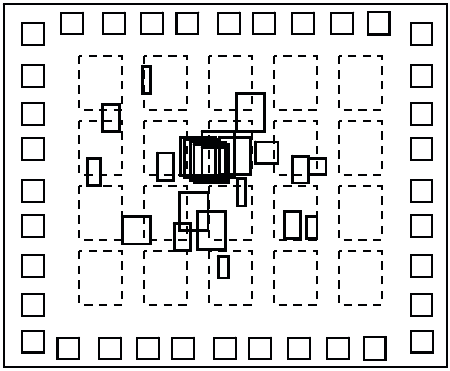
\includegraphics[height=30mm]{analytic-placement.png}
		\label{fig:plac-a}
	}%
	\subfloat[t][complex]{
		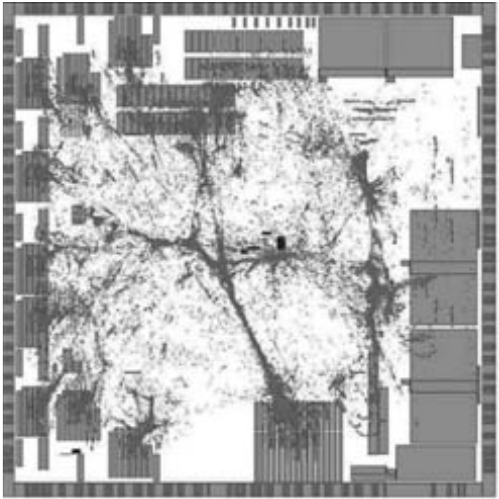
\includegraphics[height=30mm]{lots-cells.png}
		\label{fig:plac-b}
	}%
	\caption{Global placement}
	\label{fig:plac}
\end{figure}

The placer estimates some quality metrics like wire-length, wire congestion or 
signal delay. Analytics techniques can be used to model the problems as a 
minimization of an objective function via mathematical analysis.

\section{Motivation}

The cells and nets can be modeled with undirected graphs, were nodes represent 
the cells, and edges the wires. The spectral methods presented in the 
Koren~\cite{koren} paper use some properties of graphs to place each node, while 
a estimation of the wire-length is minimized.

The spectral methods present two major advantages compared with force directed 
methods. The global optimum can be computed efficiently, and the energy function 
contains $O(|E|)$ instead of $O(|V|^2)$ entries.
% TODO: Expand

\section{Methods}

Two main methods are presented, using the Laplacian matrix $L$ and a normalized 
version. Let the undirected graph $G = (V, E)$ be represented by the adjacency 
matrix $A$, defined as
\begin{equation}
A(i,j) =
\begin{cases}
	1 & \text{if $i$ and $j$ are connected} \\
	0 & \text{otherwise}
\end{cases}
\end{equation}
Let the degree of a node $i$ be defined as $d_i$, and the degree matrix $D$ with 
the degree of each node in the diagonal, $D(i,i) = d_i$ and zeros elsewhere.  

\subsection{Method 1: Laplacian matrix}

The problem is then formulated as the minimization of the squared wire-length.  
Let $x(i)$ be the position in the horizontal axis of the node $i$.
%
\begin{equation}
\begin{split}
\min_x \  & E(x) = \sum_{(i,j) \in E} (x(i) - x(j))^2 \\
\textrm{given} \ & \textrm{Var}(x) = 1
\end{split}
\end{equation}
%
The energy to be minimized $E(x)$ tries to reduce the distance between nodes, 
while the variance $\textrm{Var}(x)$ keeps the nodes from collapsing into a 
single point. The problem can be rewritten using the Laplacian matrix $L$, 
defined as $L = D - A$ or also written
%
\begin{equation}
L(i,j) =
\begin{cases}
	d_i & \text{if $i = j$} \\
	-1 & \text{if $i$ and $j$ are connected} \\
	0 & \text{otherwise}
\end{cases}
\end{equation}
%
So we finally get
%
\begin{equation}
\begin{split}
\min_x \  & x^T L x \\
\textrm{given} \ & x^T x = 1 \\
\textrm{in the subspace} \ & x^T \cdot 1_n = 0 \\
\end{split}
\end{equation}
%
Were the solution for $x$ is computed by solving the eigenproblem $L u_i = 
\lambda_i u_i$. The horizontal positions of the nodes are given by $x = u_2$.

The vertical coordinates can be obtained by using the next eigenvector $y = 
u_3$, which is orthogonal to $x$.

\subsection{Method 2: Normalization}

A slight modification of the model can lead to more interesting results. Nodes 
with high degree should be placed at the center, in order to reduce the costs of 
their multiple edges. In the following model
%
\begin{equation}
\begin{split}
\min_x \  & \frac{x^T L x}{x^T D x} \\
\textrm{in the subspace} \ & x^T D 1_n = 0 \\
\end{split}
\end{equation}
%
the numerator places the high degree nodes close to the center, while the 
denominator tries to scatter them away. As a result, the graph is more balanced, 
avoiding low degree nodes placed far away.

The solution of this new model can be obtained by solving the following 
generalized eigenproblem:
%
\begin{equation}
L u_i = \lambda_i D u_i
\end{equation}
%
And using the associated eigenvector $u_2$ of the second lowest eigenvalue 
$\lambda_2$ we get the horizontal positions of the nodes $x = u_2$. For the 
vertical positions we use the third eigenvector, $y = u_3$.

\section{Results}

In order to test and compare the results of the two algorithms, the method of 
force-directed placement \cite{forces} using attractive and repulsive forces was 
also included for comparison.

Three graphs of increasing size were used. Graph $A$ was hand generated, to test 
the placement by inspecting the intermediate matrices. The graph $B$ is a random 
Erdös-Renyí graph with 100 nodes and $p=0.1$. Finally, a real circuit was 
generated from a Verilog example, and synthesized by the open tool Yosys 
\cite{wolf} of the IceStorm project, using the Lattice iCE40 FPGA as the target.  
This final graph $C$ contains 345 nodes.

The wire-length was computed as the sum of Euclidean length of the edges, and 
the positions have been scaled to have standard deviation $\sigma = 1$, so that 
we can compare wire-length under the same dimensions.
%
% TODO: Discuss
The method of using a square bounding box of unit area to scale the graph was 
rejected, as it can lead to great reduction in wire-length if a few nodes are 
placed very far away.

Results are shown for the three graphs in the figures~\ref{fig:graphA} 
\ref{fig:graphB} and \ref{fig:graphC}, using the three methods previously 
described.

\begin{figure}[h]
	\centering
	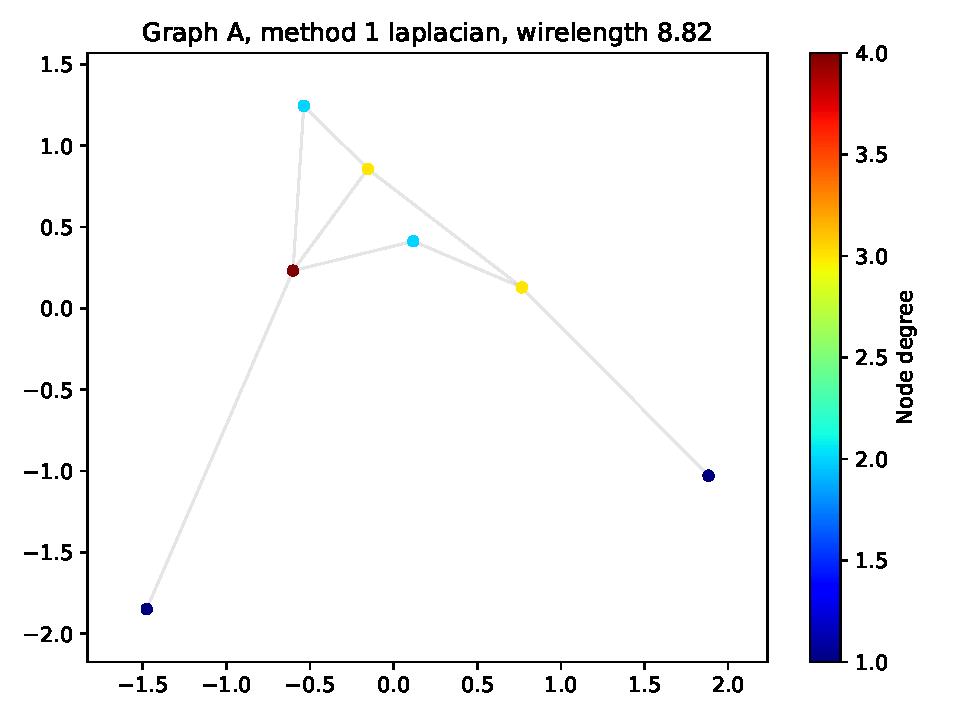
\includegraphics[width=\columnwidth]{fig/A/laplacian.pdf}
	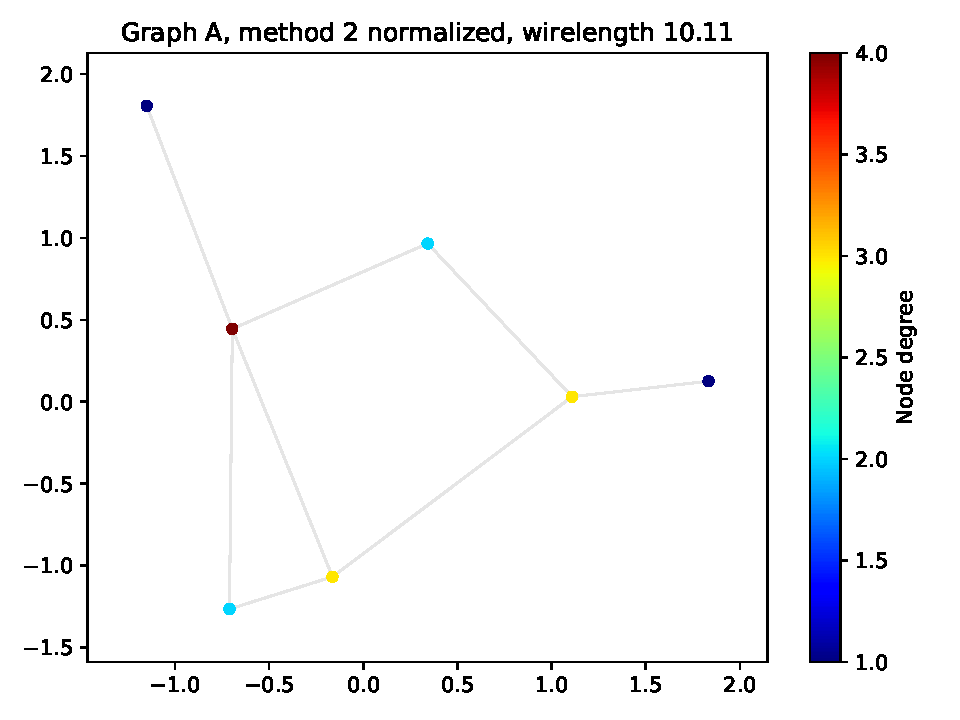
\includegraphics[width=\columnwidth]{fig/A/norm.pdf}
	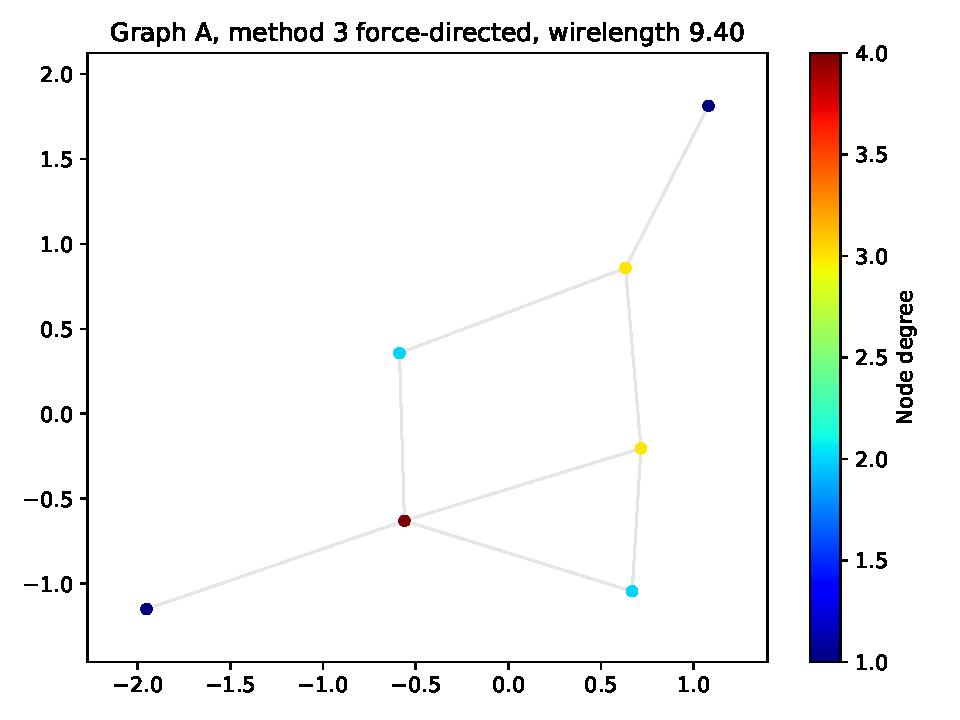
\includegraphics[width=\columnwidth]{fig/A/spring.pdf}
	\caption{Placement of graph A}
	\label{fig:graphA}
\end{figure}

\begin{figure}[h]
	\centering
	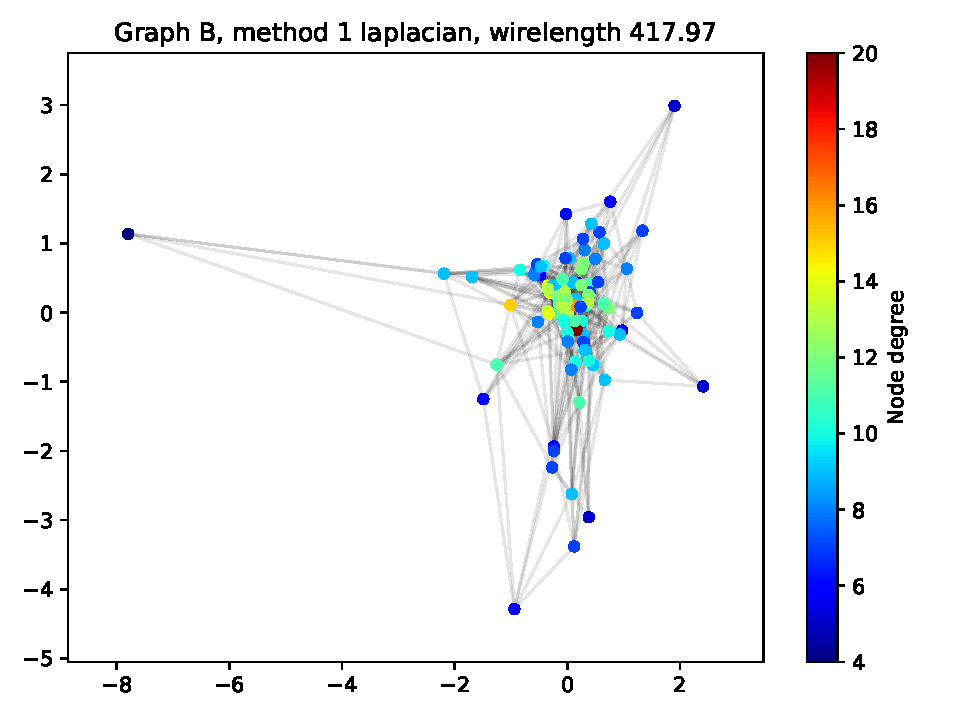
\includegraphics[width=\columnwidth]{fig/B/laplacian.pdf}
	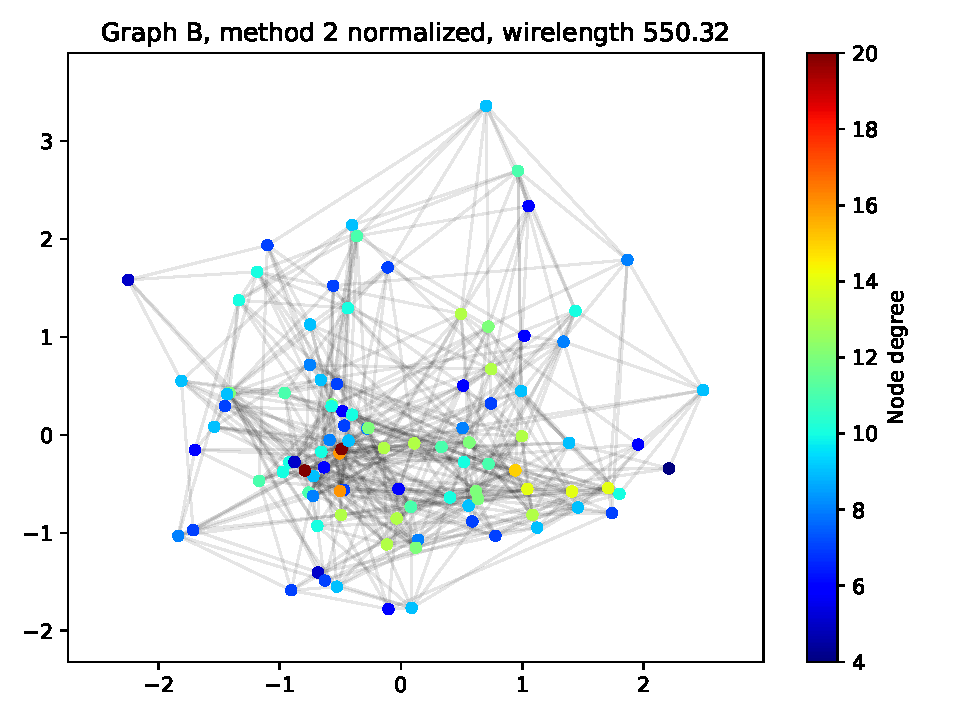
\includegraphics[width=\columnwidth]{fig/B/norm.pdf}
	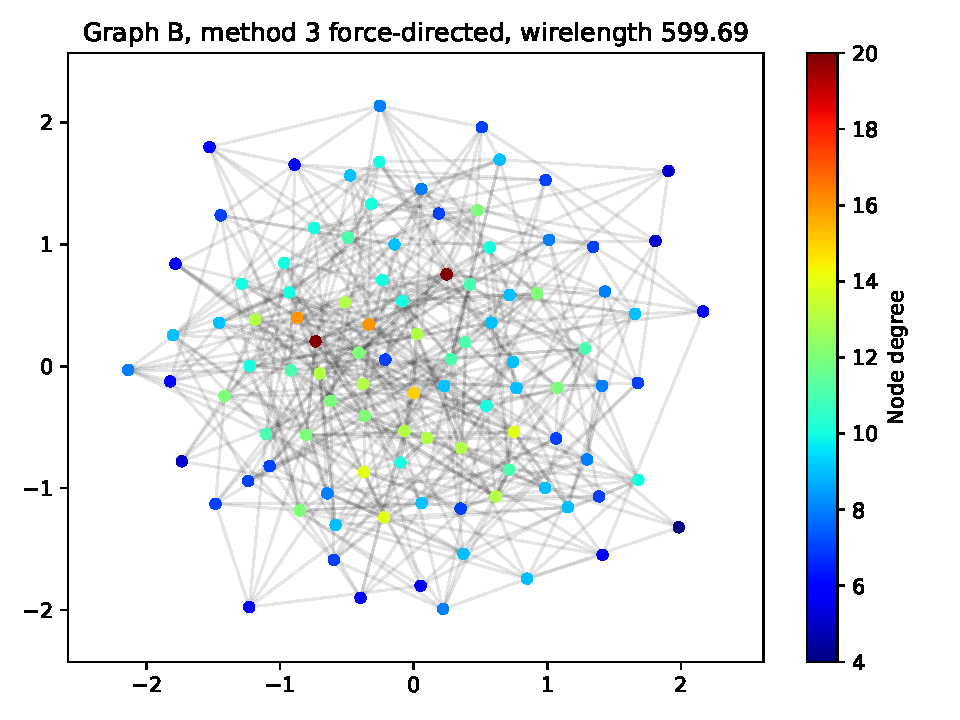
\includegraphics[width=\columnwidth]{fig/B/spring.pdf}
	\caption{Placement of graph B}
	\label{fig:graphB}
\end{figure}

\begin{figure}[h]
	\centering
	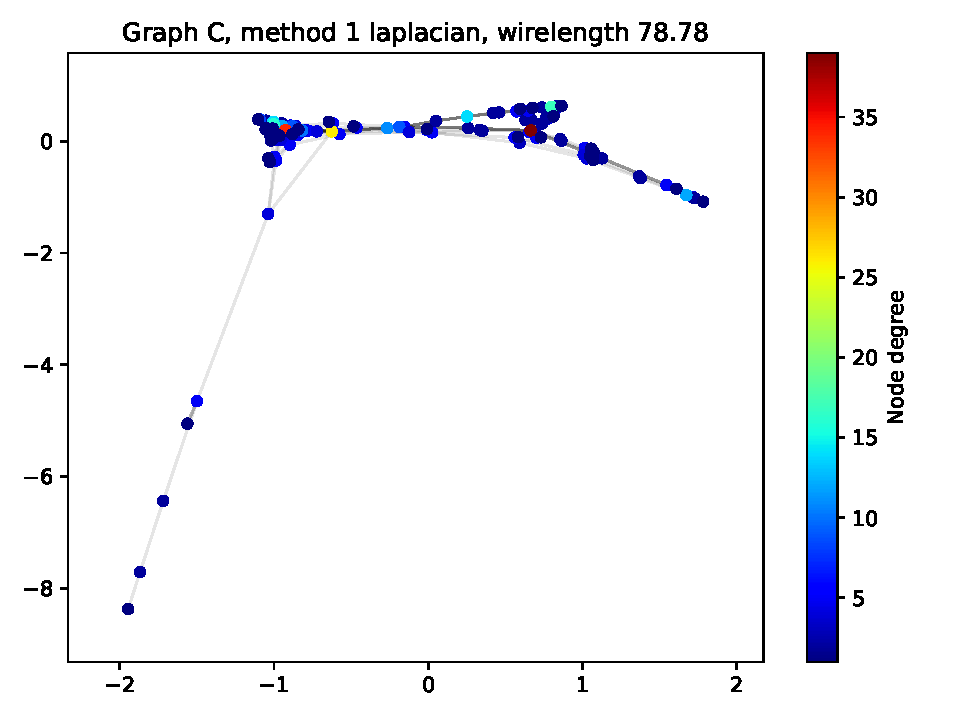
\includegraphics[width=\columnwidth]{fig/C/laplacian.pdf}
	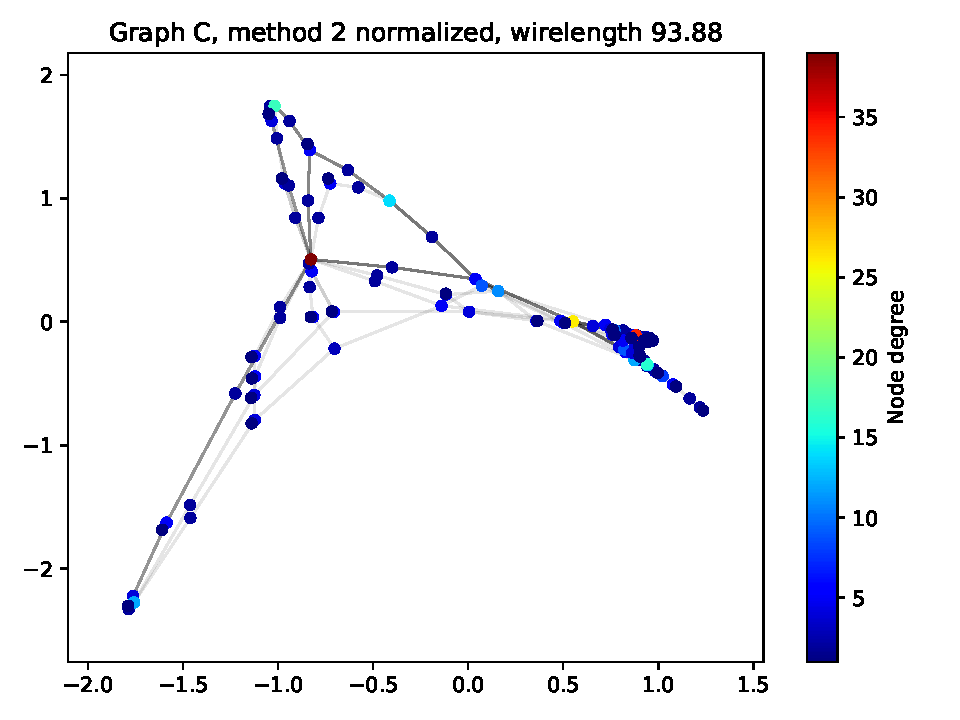
\includegraphics[width=\columnwidth]{fig/C/norm.pdf}
	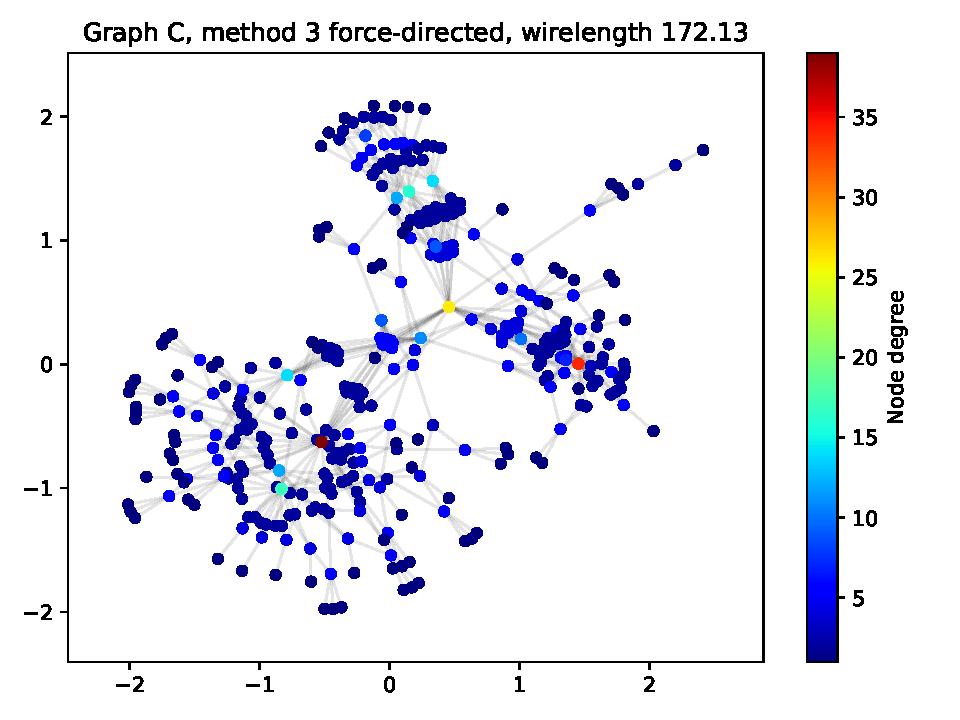
\includegraphics[width=\columnwidth]{fig/C/spring.pdf}
	\caption{Placement of graph C}
	\label{fig:graphC}
\end{figure}

\section{Discussion}

In the graph A show in the figure~\ref{fig:graphA}, we see how the three methods 
produce similar results, with the Laplacian method giving the lower wire-length.  

The figure~\ref{fig:graphB} shows a more interesting pattern. All high degree 
nodes are placed in the center, in the three methods. However, the Laplacian 
method gives a layout with a lot of overlapping nodes, with high variability in 
the node edges. A few low degree nodes were placed very far away. The method 2, 
deals with this problem, by placing the nodes in a more uniform way, while 
keeping the high degree nodes in the center. In terms of wire-length, the 
Laplacian is still getting the best result, but methods 2 and 3 seem more 
reasonable in a realistic problem.

The final graph C, shown in figure~\ref{fig:graphC} shows a different network, 
with large chains of low degree nodes. Similarly, we see a lot of overlapping 
nodes with the first method, but more sparse using the method 2, while the 3 has 
a more uniform distance between nodes, but the worst wire-length.

We see some nodes in the placements given by the Laplacian method, about 8 units 
away from the center $(0,0)$, for graphs $B$ and $C$. However, if we scale the 
graphs to fit the unit square, we reduce the wire-length up to half the size, 
compared to the method 2. Because of this problem, the graphs were scaled to 
have standard deviation $\sigma = 1$, allowing some outlier nodes to be far away 
from the graph.

\section{Conclusions}

We see that the Laplacian method produces a very short wire-length solution, but 
by using a lot of overlapping nodes. The normalized method has a behaviour 
closer to the real limitations, similarly to the force-directed method, while 
keeping the wire-length shorter.

Additionally, the algorithm provided in the Koren paper \cite{koren}, based on 
the power iteration, can be used to extract only the needed eigenvectors, 
leading to an efficient method of obtaining the global minimum.

Followed by a fine placement step, the normalized method seems to be suitable 
for larger graphs.

\bibliographystyle{siam}
\bibliography{report}

\newpage

\appendix

\section{Comment}

In the presentation of this project, the code used to plot the normalized 
Laplacian method was incorrect. As a result, the graphs shown had nodes with 
high degrees away from the center.

Two different methods were used to test for consistent results, with two 
different bugs that lead to the same wrong graph.  One of the method presented 
used the normalized Laplacian matrix $\mathcal L$, but was excluded from this 
report, as the actual explanation is simpler. After a long debugging process, 
both bugs were found and fixed. The presented graphs now are consistent with the 
expected results, giving a placement with high degree nodes in the center.

\end{document}
